\documentclass{article}
\usepackage{amsmath}
\usepackage{booktabs}
\usepackage{graphicx}

\title{Design Write Up test}
\author{Graham Pellegrini}
\date{\today}


\begin{document}
\maketitle
\section{Line output to ADC Circuit (input)}
The issue faced and previously discussed was the need to convert the line level output recived from the headphone jack to a voltage level that can be read by the ADC. \\

On implementation of the required circuit, the respective components were acuired and the circuit was assembled following the schematic provided. The circuit was tested with an oscilloscope to ensure that the output was being centered correctly between the 0 and $V_{ref}$ levels. Testing before trying to connect directly to the microcontroller was done to ensure that no damage would be done to the microcontroller and the adc components.\\

The inital implementation of the circuirt indeed did not work fully as expected, due to one of the 1N4148 diodes being blown out. This initially lead to the belief that the diodes orientation were incorrect. However, after testing the diodes seperately and replacing the blown diode, the circuit was tested again and the output was as expected. 

\begin{figure}[htpb]
    \centering
    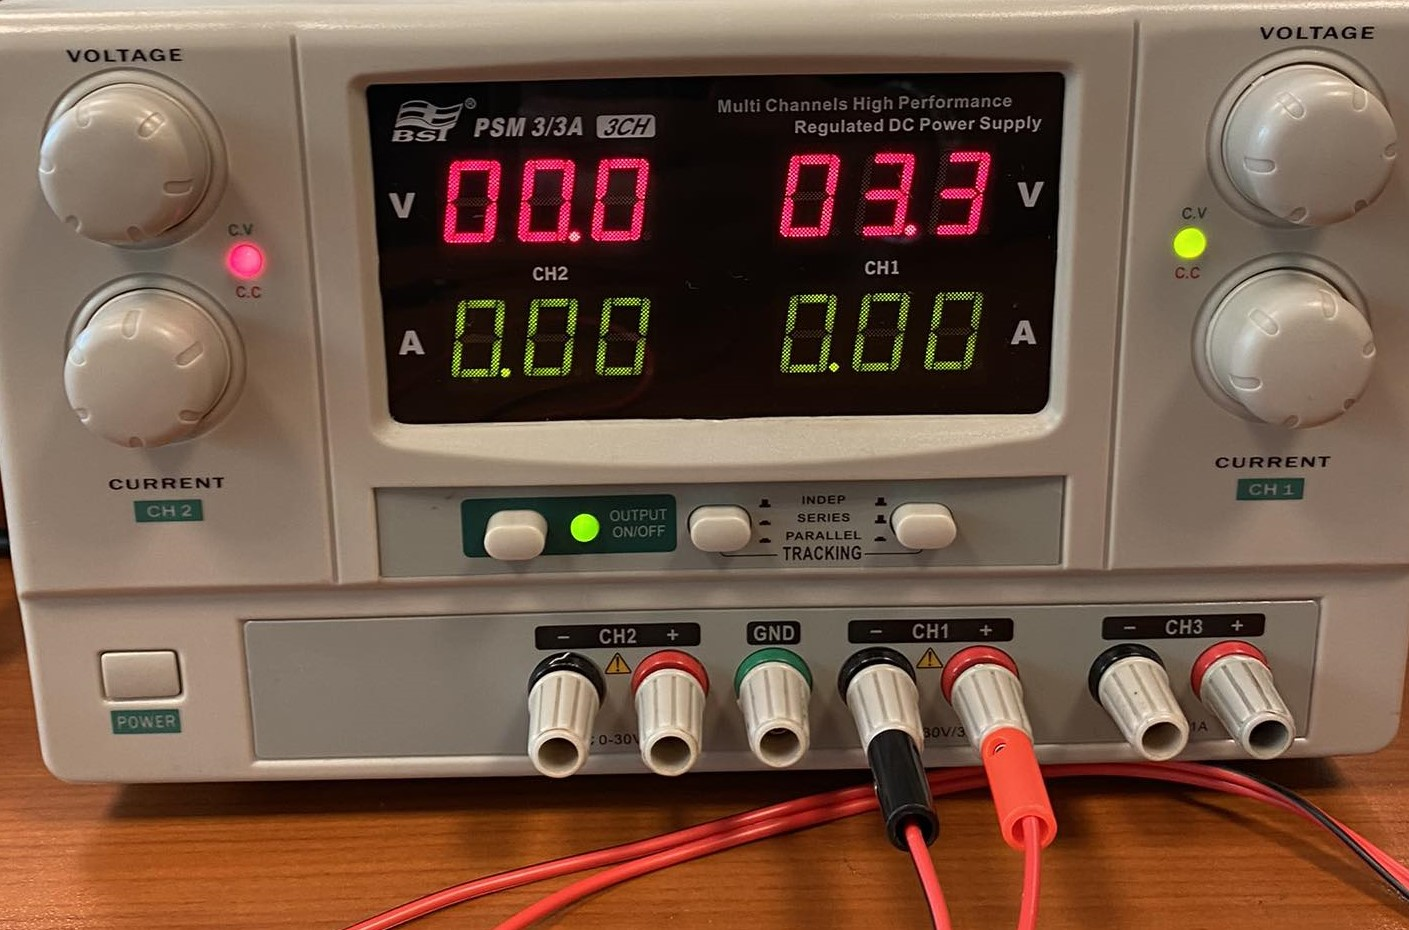
\includegraphics[width=0.7\linewidth]{vref.jpg}
    \caption{Voltage Supply set for Vref}
    \label{fig1}
\end{figure}

\begin{figure}[htpb]
    \centering
    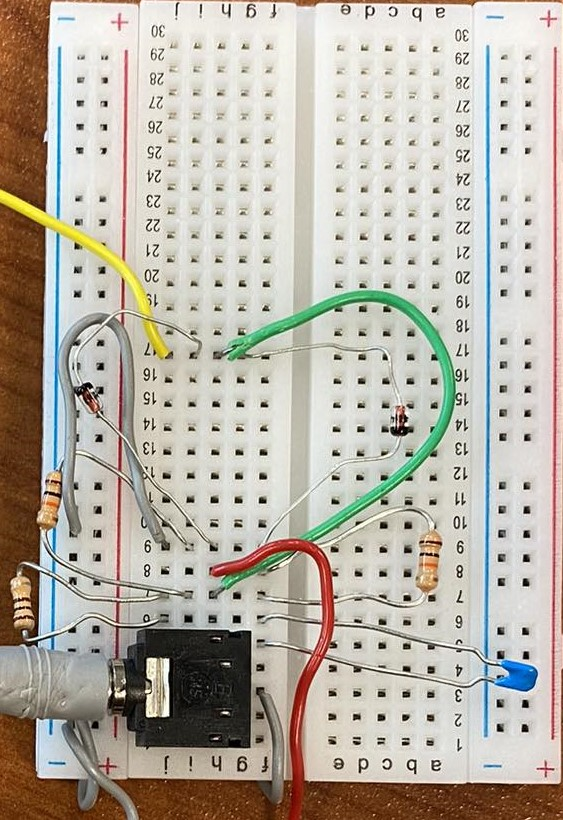
\includegraphics[width=0.8\linewidth]{circuit.jpg}
    \caption{Circuit Implementation}
    \label{fig2}
\end{figure}

\begin{figure}[htpb]
    \centering
    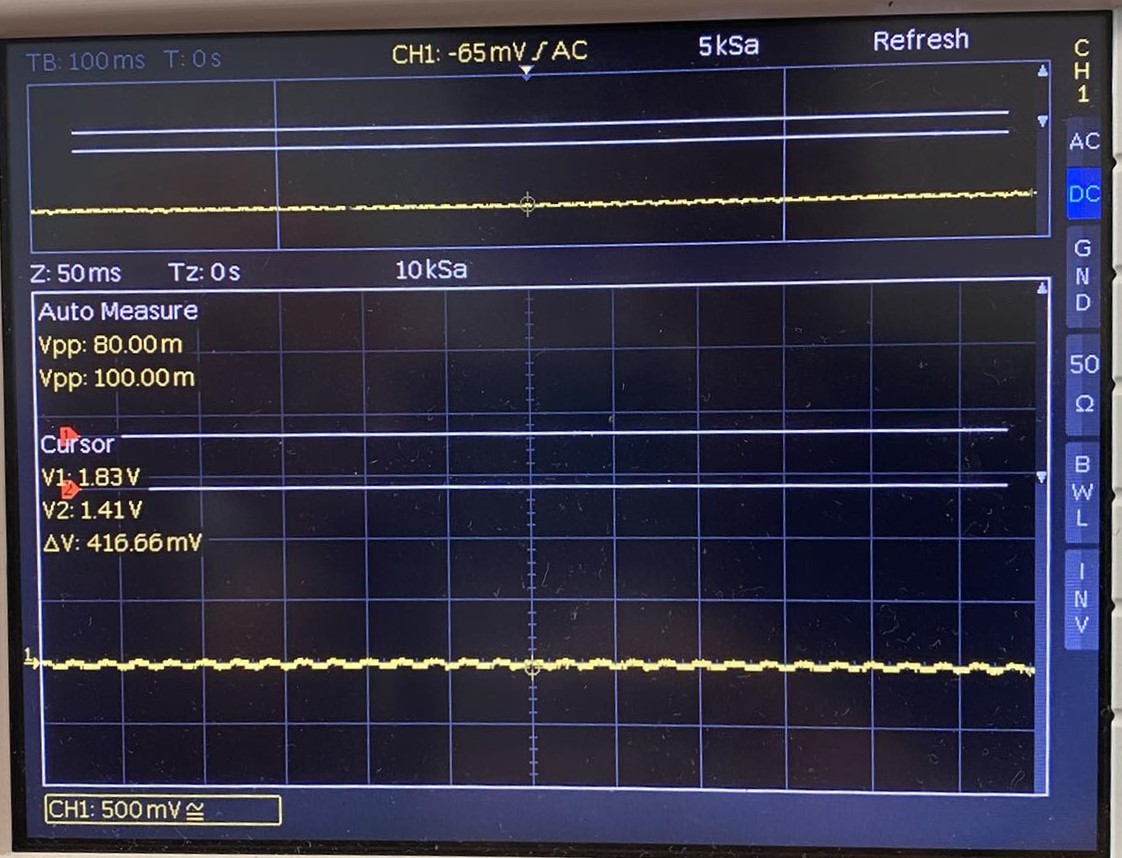
\includegraphics[width=0.8\linewidth]{shifted_difference.jpg}
    \caption{Circuit Implementation}
    \label{fig3}
\end{figure}

In figure \ref{fig3}, the output of a quite region without the respective circuirt connections is shown. In the plot, the cursor indicates the required region that the output should be centered around. However, it is clear that the output is not centered around the required region.

\begin{figure}[htpb]
    \centering
    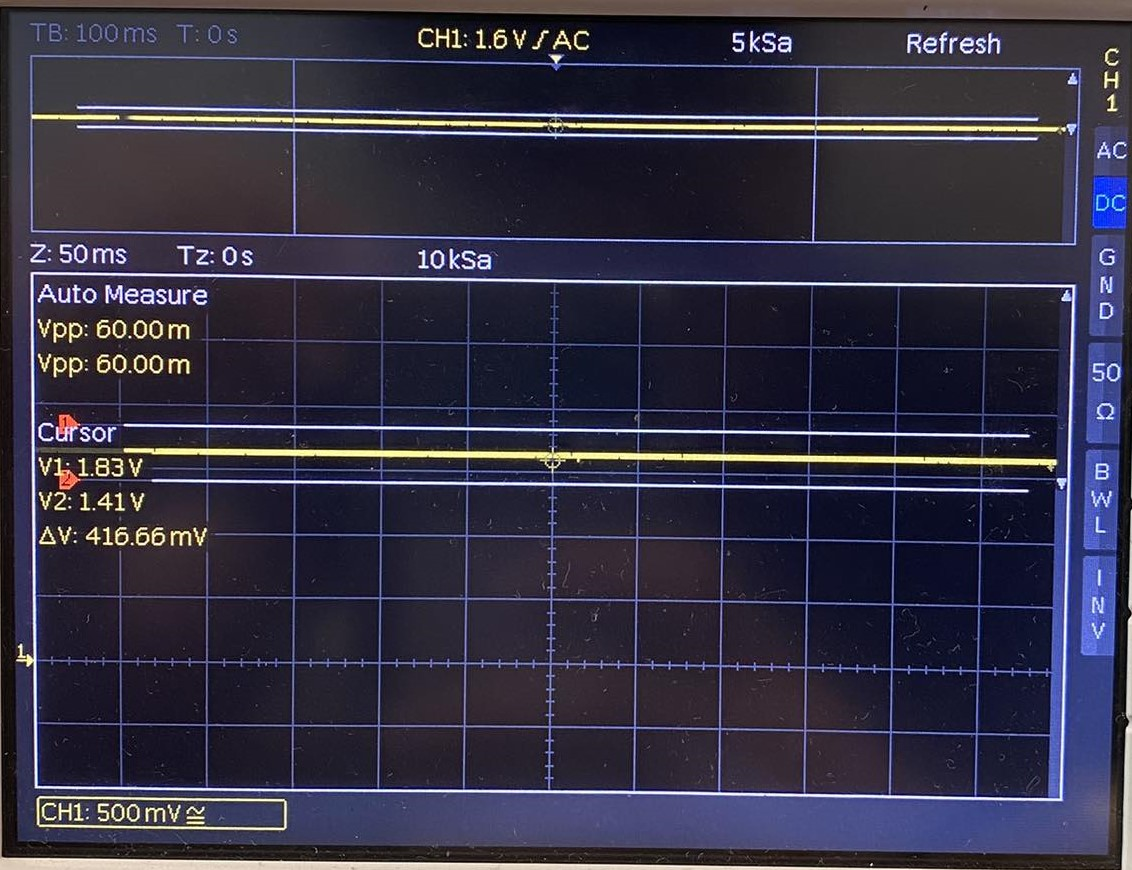
\includegraphics[width=0.8\linewidth]{quite_shifted.jpg}
    \caption{Circuit Implementation}
    \label{fig4}
\end{figure}

In figure \ref{fig4}, we can see the same quite signal with the circuit connected. The output is now centered around the required region. Indicating that the circuit is working as expected and that the output signal should be able to be read by the ADC.


\begin{figure}[htpb]
    \centering
    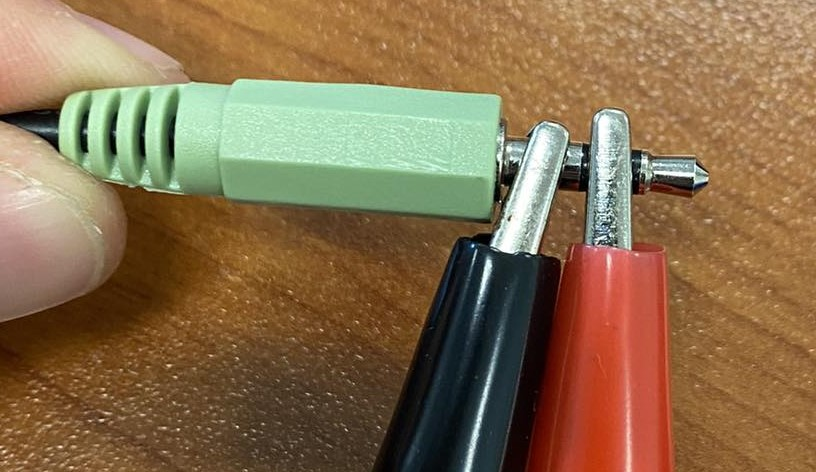
\includegraphics[width=0.8\linewidth]{jack_connections.jpg}
    \caption{Jack Connections}
    \label{fig5}
\end{figure}

In figure \ref{fig5}, the direct connection of the headphone jack output to the oscilloscope is shown. This is done by identitfying the left,right and ground connections of the headphone jack and connecting the respective oscilloscope probes to the ground and right/left connections. Knowing that the output is a stereo signal, the left and right channels were tested seperately, but results were the same.

\begin{figure}[htpb]
    \centering
    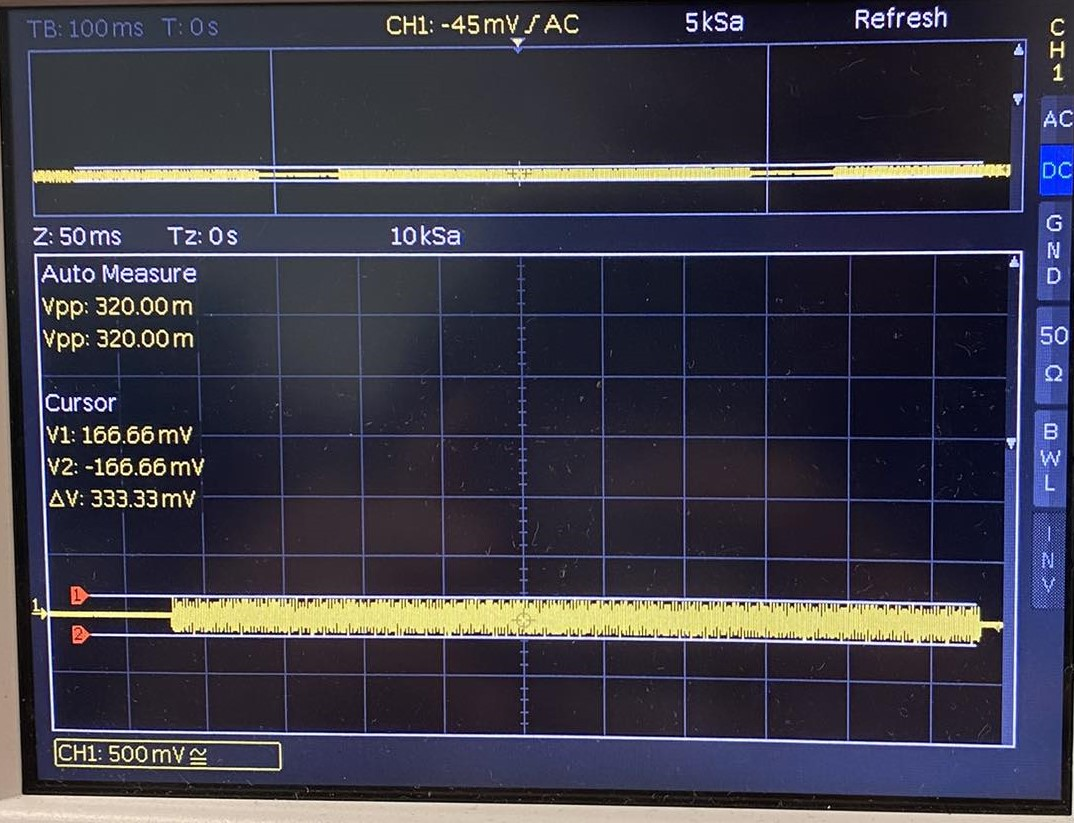
\includegraphics[width=0.8\linewidth]{signal_unshifted.jpg}
    \caption{Unshifted Signal}
    \label{fig6}
\end{figure}

In figure \ref{fig6}, the output of a signal being played through the headphone jack connection is shown in figure \ref{fig5}. The output is not centered around the required region and the signal is not able to be read by the ADC. 

\begin{figure}[htpb]
    \centering
    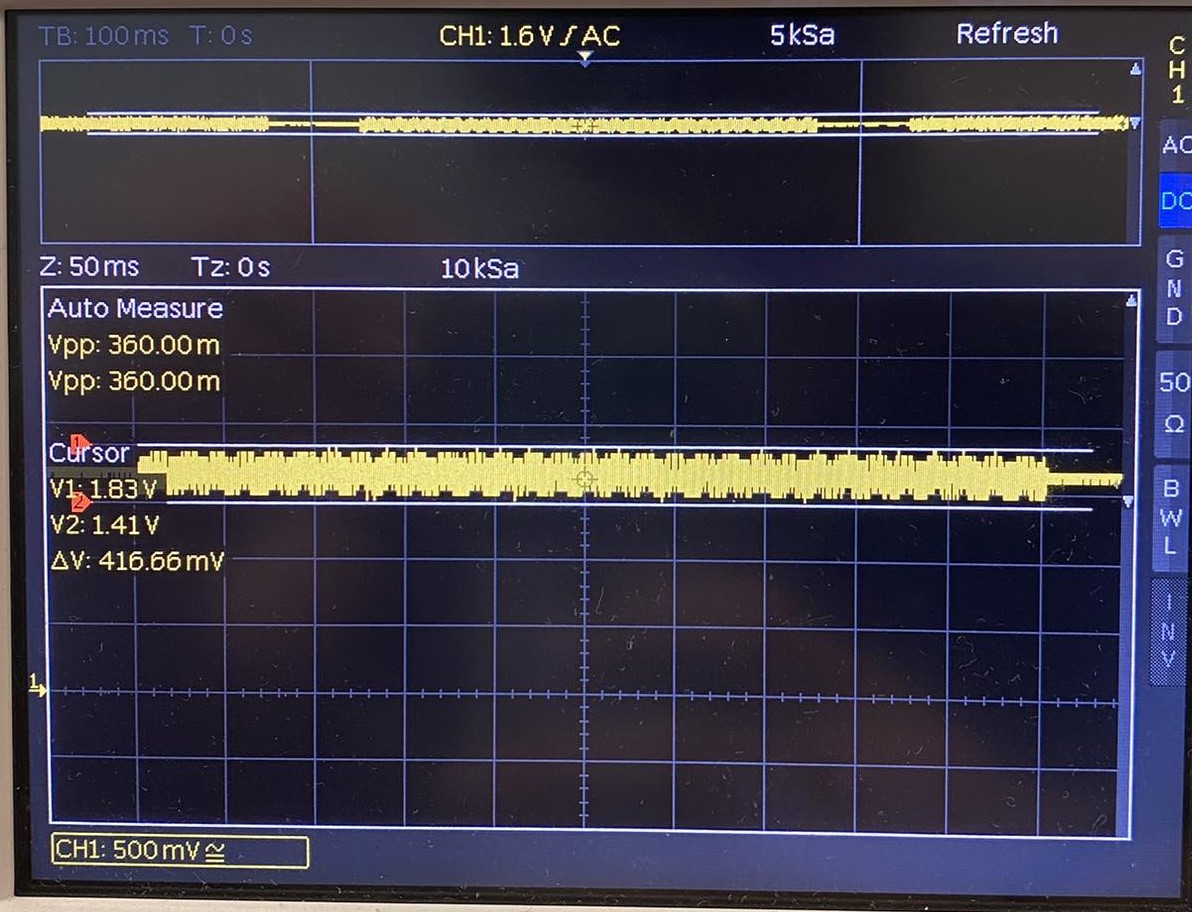
\includegraphics[width=0.8\linewidth]{signal_shifted.jpg}
    \caption{Shifted Signal}
    \label{fig7}
\end{figure}

In figure \ref{fig7}, the output of a signal is now connected to the circuit. Comparing to figure \ref{fig6}, the output is now centered around the required region and the signal is able to be read by the ADC. However, in both figures it was noted that the signal power recived is relatively low. This is due to the player properties at the laptop output, even when the volume is set to max. A solution to this was to use a different source player such as an mp3 player or phone with a higher output power. The implementation of a amplifier in the circuit was also discussed. However, the adc was still able to read the signal and the power was sufficient for the purposes of the project. Therefore, the complication of adding an amplifier was not persued, in order to keep the circuirt as simple as possible. This was an engineering desicion made to keeping the project within scope and simplicity.

\begin{figure}[htpb]
    \centering
    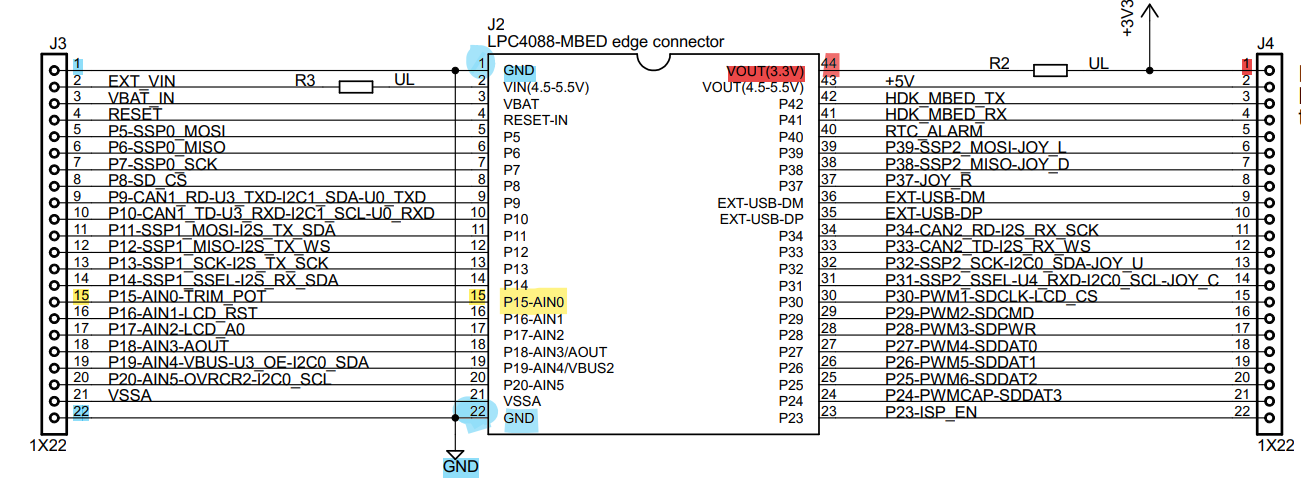
\includegraphics[width=0.8\linewidth]{pin_config.png}
    \caption{Pin Configuration}
    \label{fig8}
\end{figure}

\begin{figure}[htpb]
    \centering
    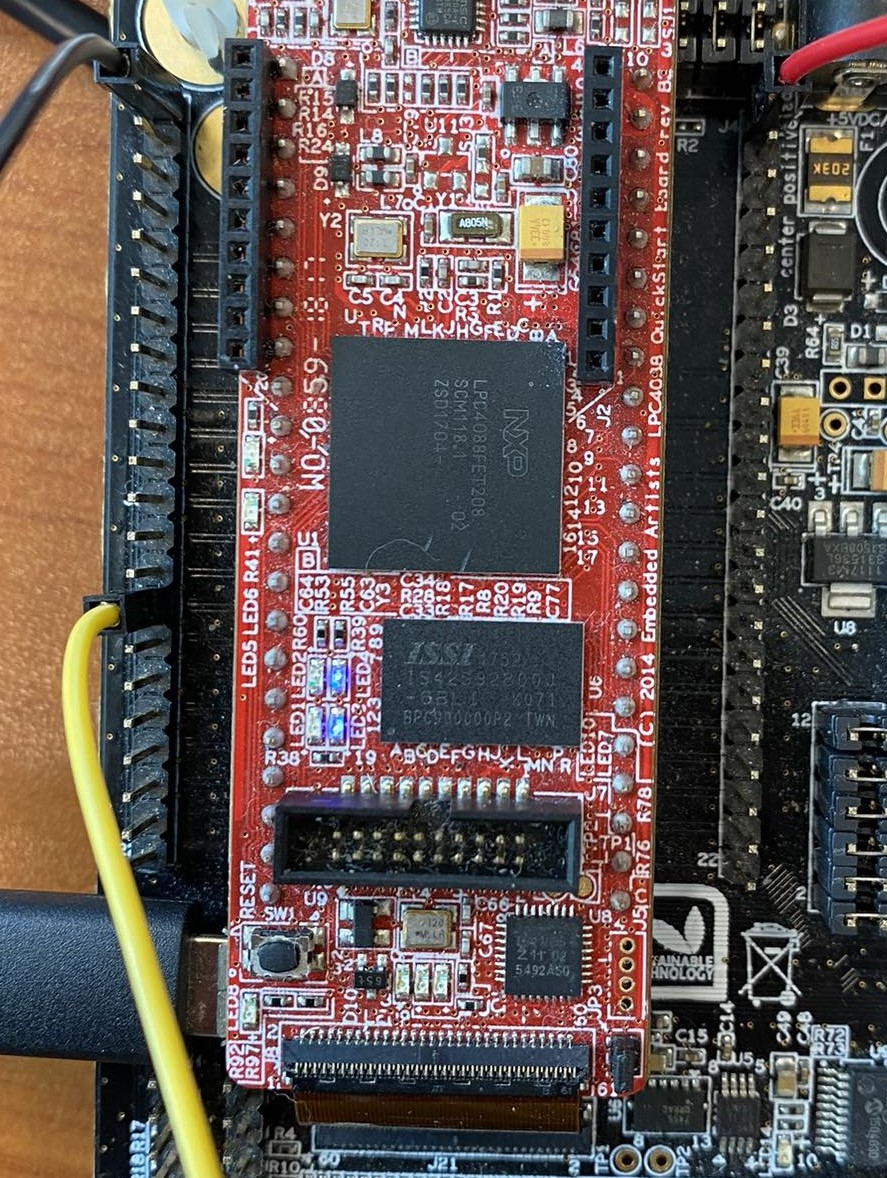
\includegraphics[width=0.6\linewidth]{board_connections.jpg}
    \caption{On Board Connections}
    \label{fig9}
\end{figure}

From the provided LPC4088 board manuals, the respective pin configurations for $V_{out}$ which is our $V_{ref}$ of 3.3, grounds and ADC in pins were identified. The pins identified are highlighted in figure \ref{fig8}. The connections were made on the board as shown in figure \ref{fig9}. The connections were made to the respective pins on the board and the circuit was tested. Having the adc properly configured and the connections made, the adc was able to read the signal and map it to the 4096 levels of the adc. The signal digital value was then printed and observed accordingly.
\pagebreak

\section{EEPROM Driver and Persistant Memory}
In the functional requirements, it was stated that a persistant storage method for a system configuration setting must be in place. This storage method must be seperate from a physical state, for instance the state of a hardware switch.But rather a read/write value that can be changed by the user and stored in memory.\\

In the ARM Cortex M4, there are two methods of persistant storage flash and EEPROM. Flash is a non-volatile memory that can be written to, but has a limited number of write cycles. EEPROM is a non-volatile memory that can be written to and has a much higher number of write cycles. The EEPROM was chosen as the persistant storage method for the project.\\

Therefore, the need for an EEPROM driver was required. The value decided on to be stored, was that of the autoscroll flag. The autoscroll flag is a boolean value that determines if the system LCD display should shift the text up and continue on a new line or clear the screen and start from the top again. The autoscroll feature is user initiated/toggled through the multi-directional switch input of an up direction. Since this value is only a flag the minimum required storage fucntionaliy of EEPROM was chosen to store the byte flag.\\

The EEPROM driver was sourced from NXP MCU SW Application Team and modified for the porject specifications. The driver fucntions included the following:

\subsection{EEPROM Initiator}
The EEPROM initiator function was used to initialize the EEPROM driver. The function was called at the start of the program to ensure that the driver works in divisions of the main system clock and to set the respective wait states for the EEPROM. 

\subsection{EEPROM Read}
The EEPROM read function was used to read the chosen address of the flag value. The function takes four parameters the eeprom page offset, the page address, the pointer to the data to be read into and the length of the data to be read.\\

The function begins by clearing the interrupt flag and setting the respective page address and offsets of the EEPROM to be read from. The EEPROM is set into read mode and an iterative loop is used to read the data into the pointer. The loop consists of waits for the EEPROM status to be ready from the read and a page overflow check. Note since we are only reading a byte from a given page the page overflow check should never be triggered, but is included for completeness of the driver. We are also only reading in the 8 bit mode of the EEPROM. However, it is caple of also reading in 16 bit and 32 bit modes. The function then returns the data read into the pointer and the autoscroll flag is read and set accordingly in the main program.

\subsection{EEPROM Write}
The EEPROM write function was used to write to the chosen address, the autoscroll flag value when updated. The function takes the same four parameters as the read function.\\

The function begins and functions very similarly to the read function. It begins by clearing the interrupt flag and setting the respective page address and offsets of the EEPROM to be written to. The EEPROM is set into write mode and an iterative loop is used to write the data from the pointer. The loop consists of waits for the EEPROM status to be ready from the write and a page overflow check. Once again since we are only writing in the 8 bit mode and only a byte is to be written, the page overflow check should never be triggered. \\

The fucntion then sets the interrupt flag to wait for the end of the program, it then sets the respective address page written to at the end and we must erase the program page to ensure that the only the data written is stored and done so correctly. The function waits till the end of the program and does not need to return any data. 

\subsection{EEPROM Erase}
The EEPROM erase function was used to erase the chosen address. The erase function is essential in EEPROM logic to ensure that the data written is the only data stored in the address. This function will preceed the write function. The function takes the page address to be erased as a parameter.\\

The function begins by setting the interrupt flag to wait for the end of the program, it then sets the respective address page to be erased. The function works by wrtitng zero to the data in the page address. The function then waits till the end of the program and does not need to return any data.

\pagebreak
\section{Error State}
Another specifications of the project was to indentitfy and indicate any error conditions that may arise. The error condition identified was the case when two high freqeucies or two low frequencies are inputed into the system. The DTMF decoder will still decode these signasl being a fourier transform function but the process will simply not be able to identify the signal. When this is the case, an error case symbol is passed through '!' the main function and the system will indicate that an error has occured. The error state is indicated by the LED flashing red and the LCD displaying a '!' symbol.\\

As previously mentioned, when an error state of such nature occures the program will not hault as the DTMF decoder still processes the freqeucies. Therefore, following an error stats and indication, the system will contiue to decode as expected keeping the same complete state it was in precceding the error state. Note when such and error is encountered, depending on how the signal is passed there might be some missed DTMF codes. That is if a DTMF signal is played in sequence with a high/low frequency producing signal. The DTMF signals at which the second signal also occurs will be missed. This is the identified error condition and the system will indicate this to the user.

\pagebreak
\section{LED Opertation}

\section{ADC Potentiometer Adjustment}




\end{document}